\documentclass[18pt]{article}
\usepackage[utf8]{inputenc}
\usepackage[a4paper, total={6.5in, 9.5in}]{geometry}
\usepackage{graphicx} % Required for inserting images
\usepackage{enumitem}
\usepackage{booktabs,adjustbox}
\usepackage{multirow,multicol}
\usepackage{xcolor}
\usepackage{array,caption}
\usepackage{amssymb,amsmath}
\usepackage{ragged2e}
\usepackage{tikz,circuitikz}
\usetikzlibrary{shapes,arrows,positioning,patterns,matrix,circuits.logic.IEC, calc}
\usepackage{pgfplots}
\pgfplotsset{compat=newest}
\usepgfplotslibrary{fillbetween,statistics}

% Source : https://tex.stackexchange.com/questions/140567/drawing-karnaughs-maps-in-latex

%isolated term
%#1 - Optional. Space between node and grouping line. Default=0
%#2 - node
%#3 - filling color
\newcommand{\implicantsol}[3][0]{
    \draw[rounded corners=3pt, fill=#3, opacity=0.3] ($(#2.north west)+(135:#1)$) rectangle ($(#2.south east)+(-45:#1)$);
    }


%internal group
%#1 - Optional. Space between node and grouping line. Default=0
%#2 - top left node
%#3 - bottom right node
%#4 - filling color
\newcommand{\implicant}[4][0]{
    \draw[rounded corners=3pt, fill=#4, opacity=0.3] ($(#2.north west)+(135:#1)$) rectangle ($(#3.south east)+(-45:#1)$);
    }

%group lateral borders
%#1 - Optional. Space between node and grouping line. Default=0
%#2 - top left node
%#3 - bottom right node
%#4 - filling color
\newcommand{\implicantcostats}[4][0]{
    \draw[rounded corners=3pt, fill=#4, opacity=0.3] ($(rf.east |- #2.north)+(90:#1)$)-| ($(#2.east)+(0:#1)$) |- ($(rf.east |- #3.south)+(-90:#1)$);
    \draw[rounded corners=3pt, fill=#4, opacity=0.3] ($(cf.west |- #2.north)+(90:#1)$) -| ($(#3.west)+(180:#1)$) |- ($(cf.west |- #3.south)+(-90:#1)$);
}

%group top-bottom borders
%#1 - Optional. Space between node and grouping line. Default=0
%#2 - top left node
%#3 - bottom right node
%#4 - filling color
\newcommand{\implicantdaltbaix}[4][0]{
    \draw[rounded corners=3pt, fill=#4, opacity=0.3] ($(cf.south -| #2.west)+(180:#1)$) |- ($(#2.south)+(-90:#1)$) -| ($(cf.south -| #3.east)+(0:#1)$);
    \draw[rounded corners=3pt, fill=#4, opacity=0.3] ($(rf.north -| #2.west)+(180:#1)$) |- ($(#3.north)+(90:#1)$) -| ($(rf.north -| #3.east)+(0:#1)$);
}

%group corners
%#1 - Optional. Space between node and grouping line. Default=0
%#2 - filling color
\newcommand{\implicantcantons}[2][0]{
    \draw[rounded corners=3pt, opacity=.3] ($(rf.east |- 0.south)+(-90:#1)$) -| ($(0.east |- cf.south)+(0:#1)$);
    \draw[rounded corners=3pt, opacity=.3] ($(rf.east |- 8.north)+(90:#1)$) -| ($(8.east |- rf.north)+(0:#1)$);
    \draw[rounded corners=3pt, opacity=.3] ($(cf.west |- 2.south)+(-90:#1)$) -| ($(2.west |- cf.south)+(180:#1)$);
    \draw[rounded corners=3pt, opacity=.3] ($(cf.west |- 10.north)+(90:#1)$) -| ($(10.west |- rf.north)+(180:#1)$);
    \fill[rounded corners=3pt, fill=#2, opacity=.3] ($(rf.east |- 0.south)+(-90:#1)$) -|  ($(0.east |- cf.south)+(0:#1)$) [sharp corners] ($(rf.east |- 0.south)+(-90:#1)$) |-  ($(0.east |- cf.south)+(0:#1)$) ;
    \fill[rounded corners=3pt, fill=#2, opacity=.3] ($(rf.east |- 8.north)+(90:#1)$) -| ($(8.east |- rf.north)+(0:#1)$) [sharp corners] ($(rf.east |- 8.north)+(90:#1)$) |- ($(8.east |- rf.north)+(0:#1)$) ;
    \fill[rounded corners=3pt, fill=#2, opacity=.3] ($(cf.west |- 2.south)+(-90:#1)$) -| ($(2.west |- cf.south)+(180:#1)$) [sharp corners]($(cf.west |- 2.south)+(-90:#1)$) |- ($(2.west |- cf.south)+(180:#1)$) ;
    \fill[rounded corners=3pt, fill=#2, opacity=.3] ($(cf.west |- 10.north)+(90:#1)$) -| ($(10.west |- rf.north)+(180:#1)$) [sharp corners] ($(cf.west |- 10.north)+(90:#1)$) |- ($(10.west |- rf.north)+(180:#1)$) ;
}

%Empty Karnaugh map 4x4
\newenvironment{Karnaugh}%
{
\begin{tikzpicture}[baseline=(current bounding box.north),scale=0.8]
\draw (0,0) grid (4,4);
\draw (0,4) -- node [pos=0.7,above right,anchor=south west] {RS} node [pos=0.7,below left,anchor=north east] {PG} ++(135:1);
%
\matrix (mapa) [matrix of nodes,
        column sep={0.8cm,between origins},
        row sep={0.8cm,between origins},
        every node/.style={minimum size=0.3mm},
        anchor=8.center,
        ampersand replacement=\&] at (0.5,0.5)
{
                       \& |(c00)| 00         \& |(c01)| 01         \& |(c11)| 11         \& |(c10)| 10         \& |(cf)| \phantom{00} \\
|(r00)| 00             \& |(0)|  \phantom{0} \& |(1)|  \phantom{0} \& |(3)|  \phantom{0} \& |(2)|  \phantom{0} \&                     \\
|(r01)| 01             \& |(4)|  \phantom{0} \& |(5)|  \phantom{0} \& |(7)|  \phantom{0} \& |(6)|  \phantom{0} \&                     \\
|(r11)| 11             \& |(12)| \phantom{0} \& |(13)| \phantom{0} \& |(15)| \phantom{0} \& |(14)| \phantom{0} \&                     \\
|(r10)| 10             \& |(8)|  \phantom{0} \& |(9)|  \phantom{0} \& |(11)| \phantom{0} \& |(10)| \phantom{0} \&                     \\
|(rf) | \phantom{00}   \&                    \&                    \&                    \&                    \&                     \\
};
}%
{
\end{tikzpicture}
}

%Empty Karnaugh map 2x4
\newenvironment{Karnaughvuit}%
{
\begin{tikzpicture}[baseline=(current bounding box.north),scale=0.8]
\draw (0,0) grid (4,2);
\draw (0,2) -- node [pos=1.3,above right,anchor=south west] {$cs_{1}$,$cs_{0}$} node [pos=0.7,below left,anchor=north east] {$cs_{2}$} ++(135:1);
%
\matrix (mapa) [matrix of nodes,
        column sep={0.8cm,between origins},
        row sep={0.8cm,between origins},
        every node/.style={minimum size=0.3mm},
        anchor=4.center,
        ampersand replacement=\&] at (0.5,0.5)
{
                      \& |(c00)| 00         \& |(c01)| 01         \& |(c11)| 11         \& |(c10)| 10         \& |(cf)| \phantom{00} \\
|(r00)| 0             \& |(0)|  \phantom{0} \& |(1)|  \phantom{0} \& |(3)|  \phantom{0} \& |(2)|  \phantom{0} \&                     \\
|(r01)| 1             \& |(4)|  \phantom{0} \& |(5)|  \phantom{0} \& |(7)|  \phantom{0} \& |(6)|  \phantom{0} \&                     \\
|(rf) | \phantom{00}  \&                    \&                    \&                    \&                    \&                     \\
};
}%
{
\end{tikzpicture}
}

%Empty Karnaugh map 2x2
\newenvironment{Karnaughquatre}%
{
\begin{tikzpicture}[baseline=(current bounding box.north),scale=0.8]
\draw (0,0) grid (2,2);
\draw (0,2) -- node [pos=0.7,above right,anchor=south west] {b} node [pos=0.7,below left,anchor=north east] {a} ++(135:1);
%
\matrix (mapa) [matrix of nodes,
        column sep={0.8cm,between origins},
        row sep={0.8cm,between origins},
        every node/.style={minimum size=0.3mm},
        anchor=2.center,
        ampersand replacement=\&] at (0.5,0.5)
{
          \& |(c00)| 0          \& |(c01)| 1  \\
|(r00)| 0 \& |(0)|  \phantom{0} \& |(1)|  \phantom{0} \\
|(r01)| 1 \& |(2)|  \phantom{0} \& |(3)|  \phantom{0} \\
};
}%
{
\end{tikzpicture}
}

%Defines 8 or 16 values (0,1,X)
\newcommand{\contingut}[1]{%
\foreach \x [count=\xi from 0]  in {#1}
     \path (\xi) node {\x};
}

%Places 1 in listed positions
\newcommand{\minterms}[1]{%
    \foreach \x in {#1}
        \path (\x) node {1};
}

%Places 0 in listed positions
\newcommand{\maxterms}[1]{%
    \foreach \x in {#1}
        \path (\x) node {0};
}

%Places X in listed positions
\newcommand{\indeterminats}[1]{%
    \foreach \x in {#1}
        \path (\x) node {X};
}
\graphicspath{ {./Util/} }

% set spacing in tables
\setlength{\tabcolsep}{12pt}
\renewcommand{\arraystretch}{1.5}


\title{
\vspace{10mm}\\
CSE 306\\
Computer Architecture Sessional\\
\vspace{10mm}\\
Assignment-2: 32-bit Floating Point Adder Simulation\\
\vspace{15mm}\\
Lab Section - A1\\
Group - 06\\
\vspace{5mm}\\
\large{22 January, 2024}\\
\vspace{20mm}
\raggedright
\Large{Members of the Group:\par}
\Large{
\begin{enumerate}[label = \roman*.]
    \item 2005020 - Mostafa Rifat Tazwar
    \item 2005025 - Most. Sonia Khatun
    \item 2005027 - Swastika Pandit
    \item 2005029 - MD. Minhajul Islam Fuad
    \item 2005030 - Fairuz Mubashwera
\end{enumerate}
}
}

\author{}
\date{}

\begin{document}

\maketitle

\newpage
\section{Introduction}
\Large
A floating point adder is a circuit that can perform addition (and subtraction) operations of
floating point numbers.Floating-point number is basically a representation of real numbers with both integer and fractional parts while working in computers.This representation can deal the numbers that are too big or too small for integer representation to deal with.

Floating point representation has three fields with fixed number of bit size : sign field, exponent field and mantissa or fraction field. Generally floating point numbers are of the form:\\
 $(-1)^{Sign} * (1+Fraction) * 2^{Exponent-Bias}$\\
 Where Bias depends on the number of bits used for representing the exponent field.If exponent field is 'e' bit then $Bias=2^{e-1}-1$\\
A floating-point adder operates by aligning the decimal points of the two numbers to be added and then adding their mantissas. The exponent of the result remains fixed, necessitating shifts and corresponding adjustments, such as incrementing or decrementing, through the normalization and rounding processes. The sign of the result is determined by the signs of the two numbers being added.

A floating-point adder finds application in diverse fields such as scientific and engineering computations, financial modeling, and computer graphics. It is employed in co-processors to execute rapid, hardware-accelerated floating-point arithmetic, particularly beneficial for computationally intensive tasks. The specialized floating-point adder exhibits superior speed compared to the main processor, proving advantageous in critical applications like scientific simulations, data analysis, and other operations demanding high-precision floating-point calculations.
\section{Problem Specification}
The assignment asks to design a floating point adder circuit which takes two floating points as inputs and provides their sum, another floating point as output. Each floating point will be 32 bits long with the following representation:
\begin{table}[!h]
    \centering
    \begin{tabular}{|p{3cm}|p{3cm}|p{3cm}|}
        \hline
         \large{\textbf{Sign}}&\large{\textbf{Exponent}}&\large{\textbf{Fraction}}  \\
         \hline
         {1 bit}&{11 bits}&{20 bits} \\
         \hline
    \end{tabular}
    \caption{Problem Specification}
    \label{tab:spec}
\end{table}
\newpage

\section{Circuit Diagram}
\begin{figure}[!h]
    \centering
    \captionsetup{font=Large}
    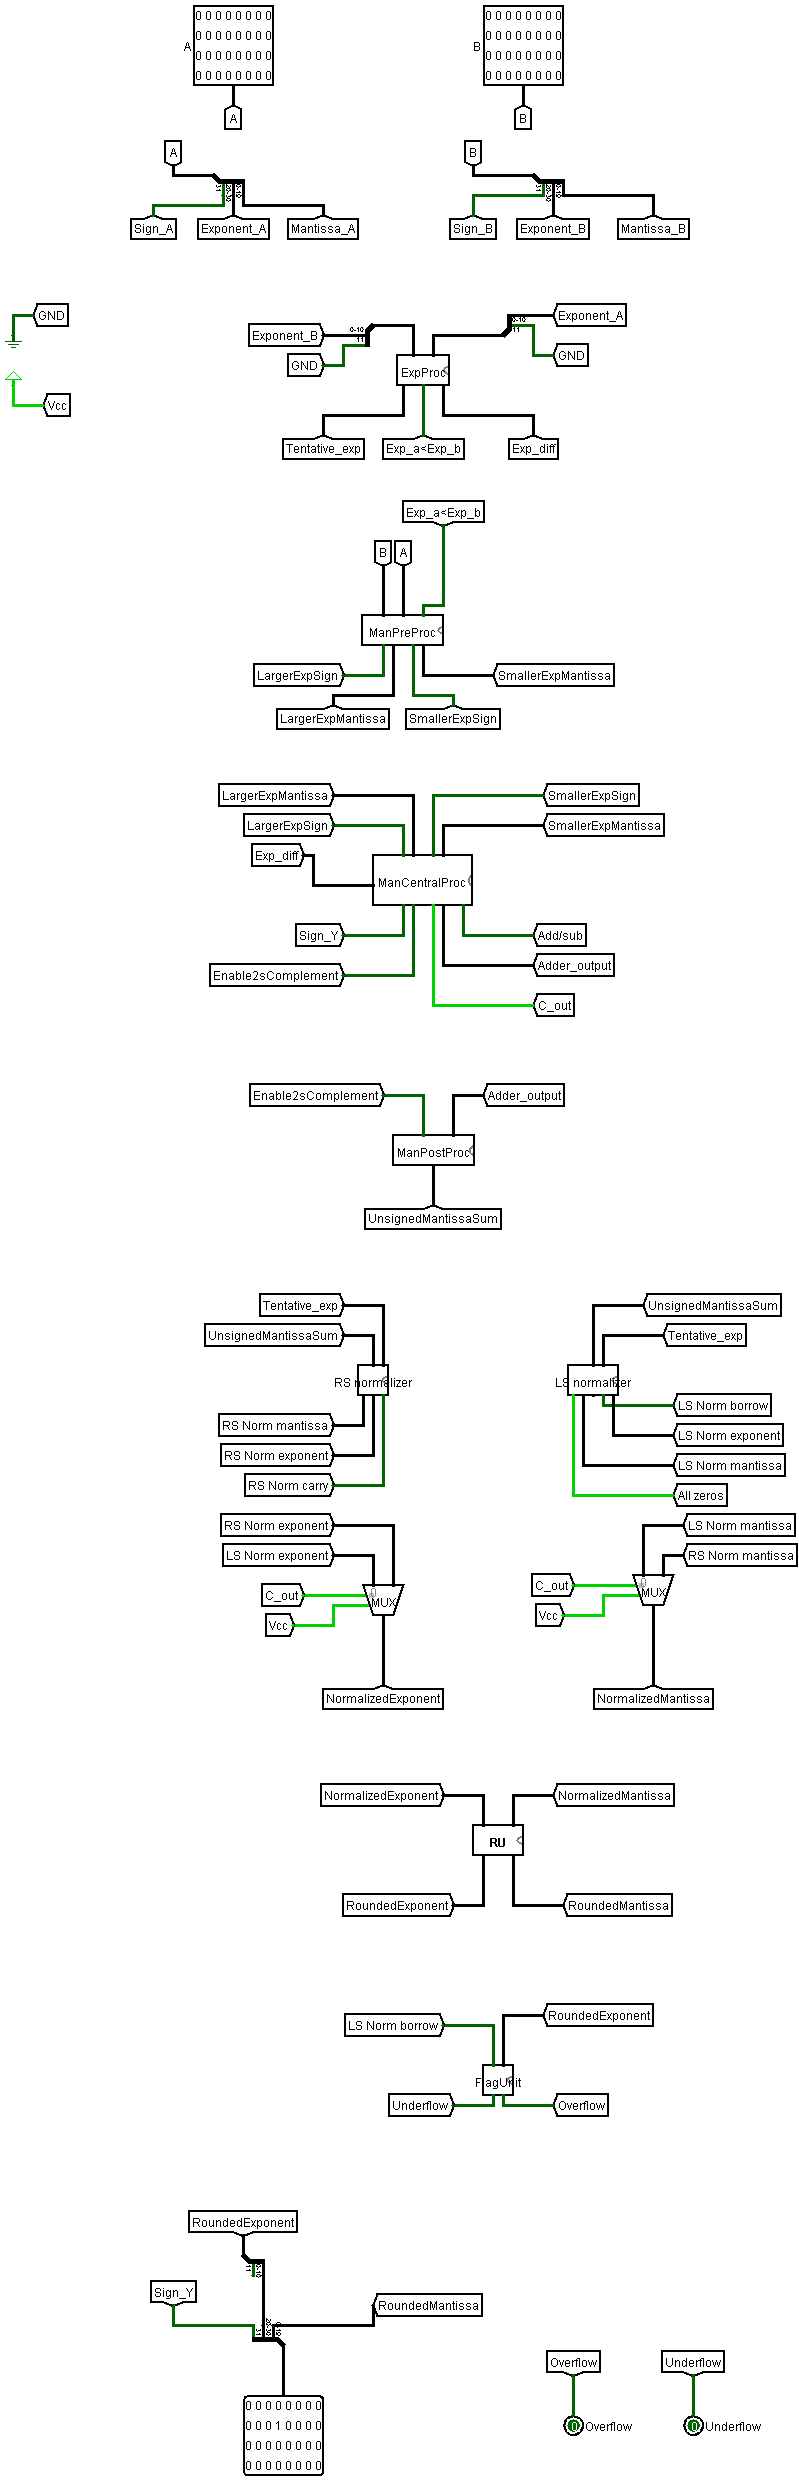
\includegraphics[scale=0.2]{Util/FPA.png}
    \caption{Flow chart of the addition/substraction algorithm}
\end{figure}
\newpage
\section{Flowchart of the Addition-Subtraction Algorithm}
\vspace{5mm}
\begin{figure}[!h]
    \centering
    \captionsetup{font=Large}
    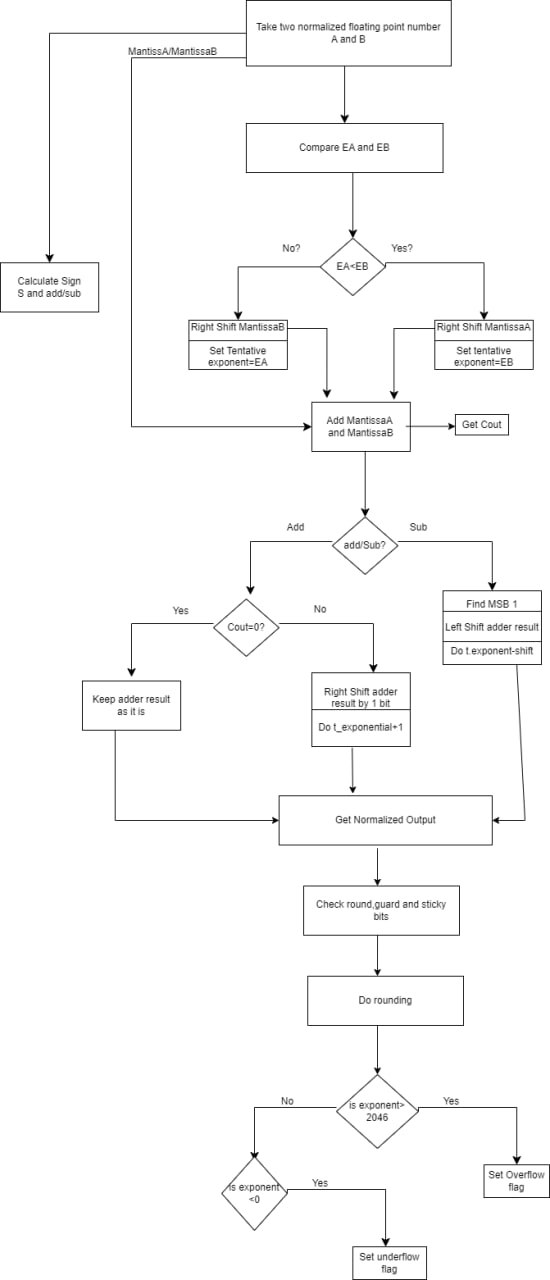
\includegraphics[scale=0.75]{Util/flowchart.jpg}
    \caption{Flow chart of the addition/substraction algorithm}
\end{figure}
\newpage
\section{Description and Circuit Diagram of Modules}
\subsection{Exponent Processor Unit}
\begin{figure}[!h]
    \centering
    \captionsetup{font=Large}
    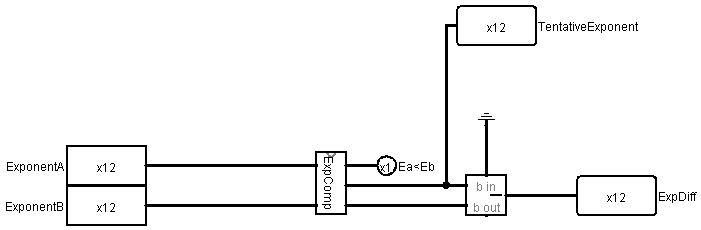
\includegraphics[scale=0.5]{Util/ExponentProcessor.png}
    \caption{ExponentProcessor.circ}
\end{figure}
\begin{figure}[!h]
    \centering
    \captionsetup{font=Large}
    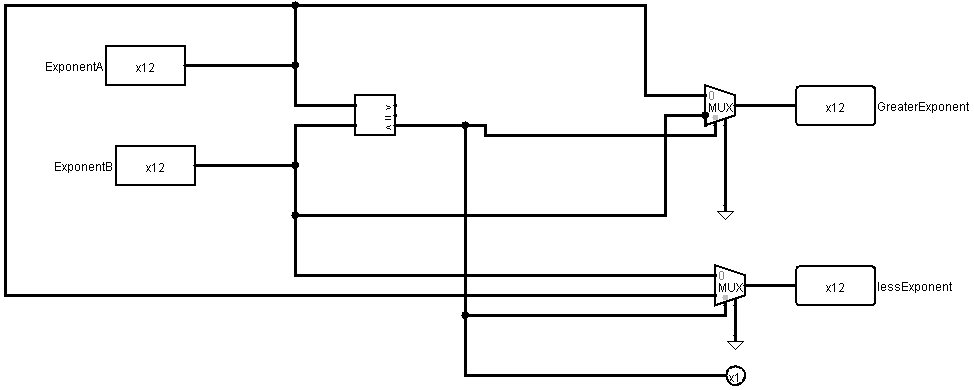
\includegraphics[scale=0.2]{Util/ExponentComparator.png}
    \caption{ExponentComparator.circ}
\end{figure}

\subsection{Mantissa Processor Unit}
\begin{figure}[!h]
    \centering
    \captionsetup{font=Large}
    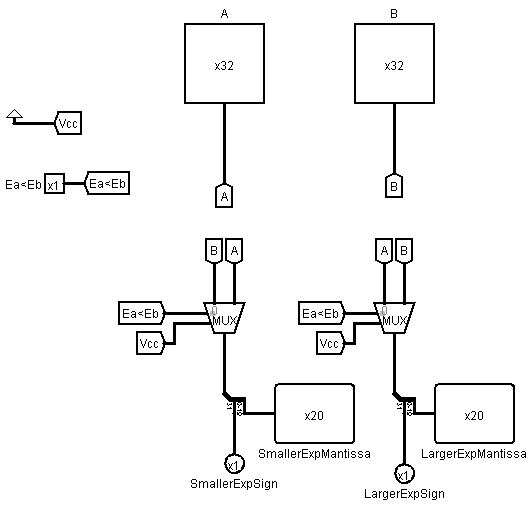
\includegraphics[scale=0.5]{Util/MantissaPreprocessor.png}
    \caption{MantissaPreprocessor.circ}
\end{figure}
\begin{figure}[!h]
    \centering
    \captionsetup{font=Large}
    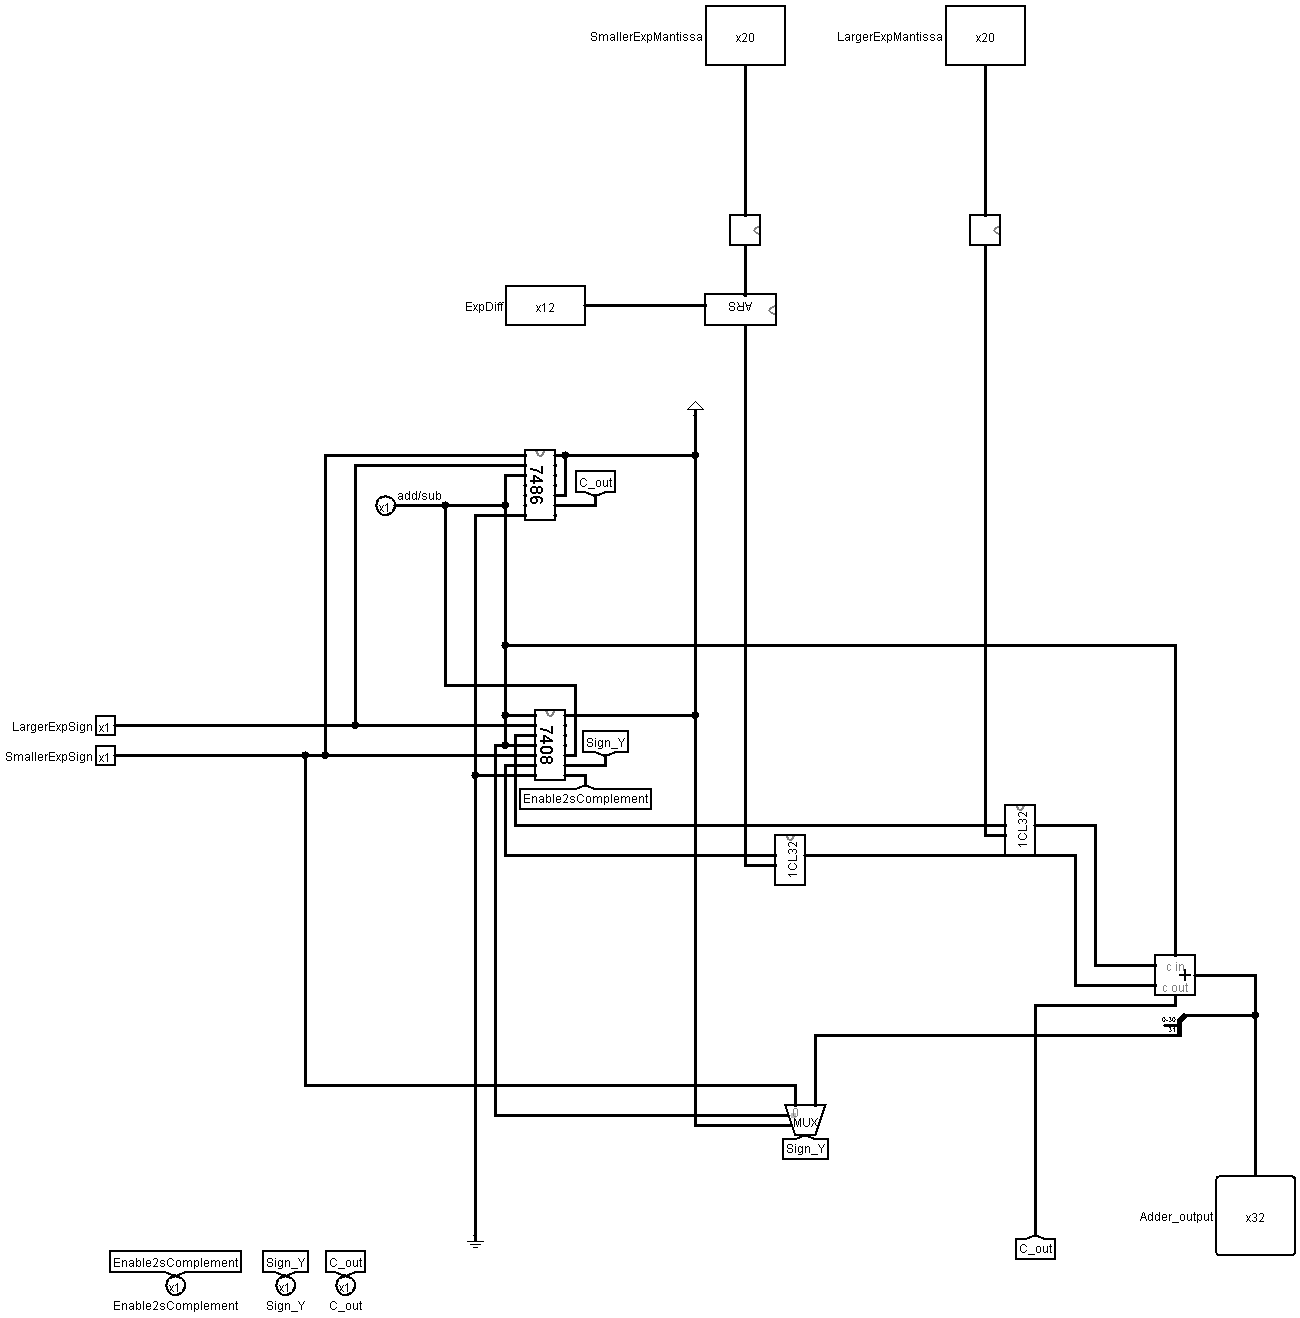
\includegraphics[scale=0.2]{Util/MantissaCentralProcessor.png}
    \caption{MantissaCentralProcessor.circ}
\end{figure}
\begin{figure}[!h]
    \centering
    \captionsetup{font=Large}
    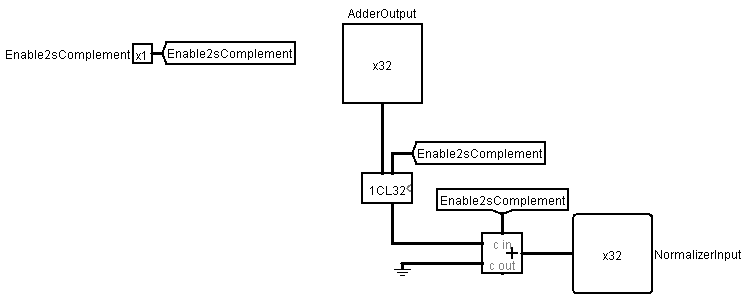
\includegraphics[scale=0.2]{Util/MantissaPostProcessor.png}
    \caption{MantissaPostProcessor.circ}
\end{figure}

\subsection{Normalizer Unit}
\begin{figure}[!h]
    \centering
    \captionsetup{font=Large}
    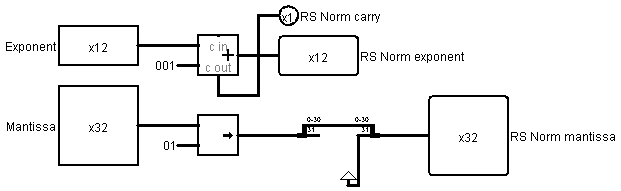
\includegraphics[scale=0.2]{Util/RS Normalizer.png}
    \caption{Right Shift Normalization.circ}
\end{figure}
\begin{figure}[!h]
    \centering
    \captionsetup{font=Large}
    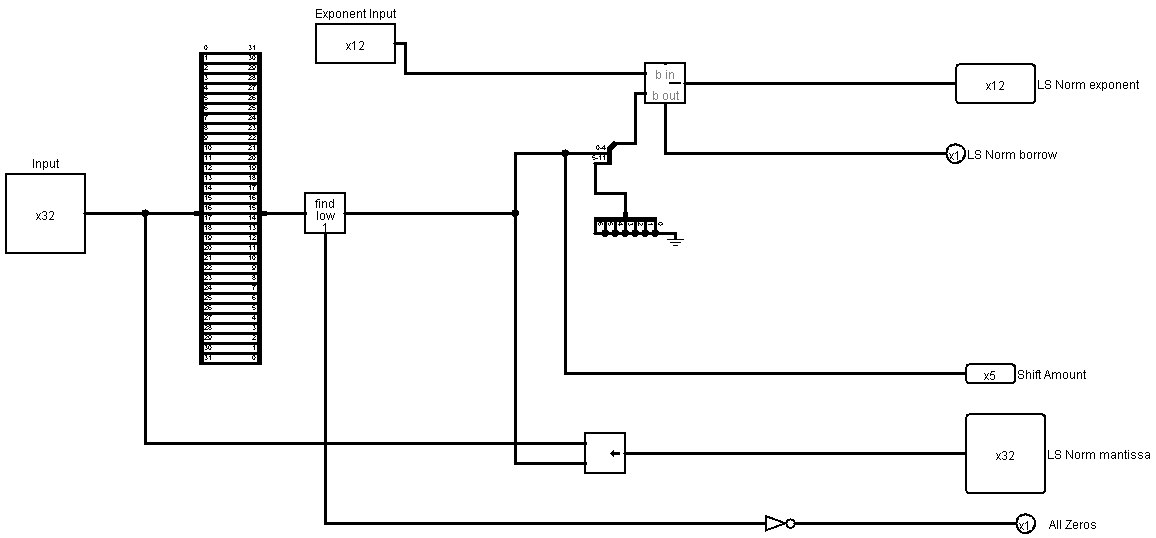
\includegraphics[scale=0.2]{Util/LS Normalizer.png}
    \caption{Left Shift Normalization.circ}
\end{figure}

\subsection{Rounding Unit}
\begin{figure}[!h]
    \centering
    \captionsetup{font=Large}
    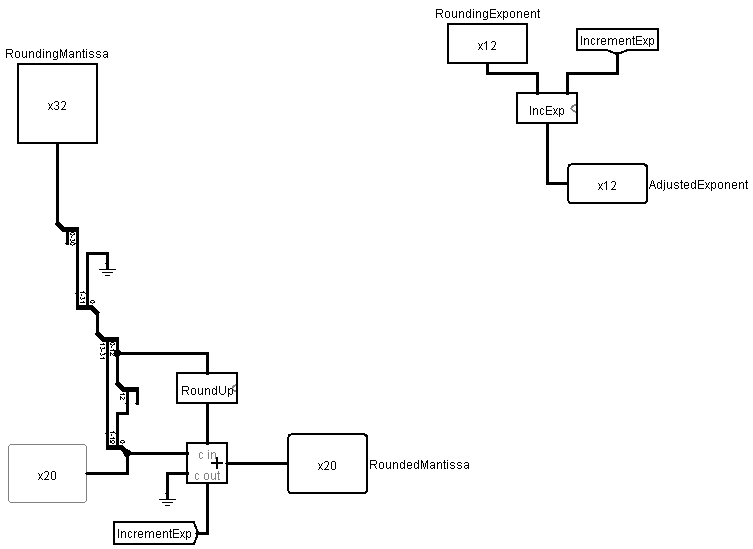
\includegraphics[scale=0.2]{Util/RoundingUnit.png}
    \caption{Rounding Unit.circ}
\end{figure}
\begin{figure}[!h]
    \centering
    \captionsetup{font=Large}
    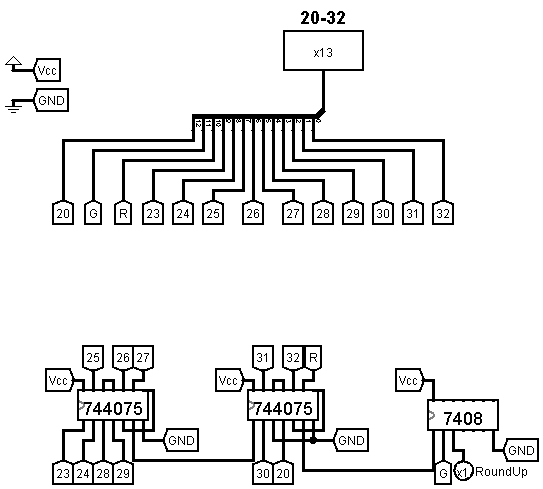
\includegraphics[scale=0.5]{Util/RoundUpFlag.png}
    \caption{Round Up Flag.circ}
\end{figure}
\begin{figure}[!h]
    \centering
    \captionsetup{font=Large}
    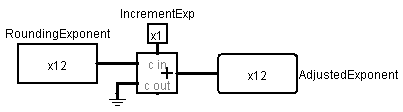
\includegraphics[scale=0.5]{Util/IncrementExponent.png}
    \caption{Increment Exponent.circ}
\end{figure}
\begin{figure}[!h]
    \centering
    \captionsetup{font=Large}
    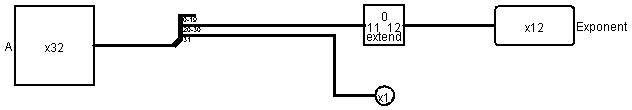
\includegraphics[scale=0.5]{Util/InitialExtractor.png}
    \caption{Initial Extractor.circ}
\end{figure}
\newpage
\subsection{Flag Unit}
\begin{figure}[!h]
    \centering
    \captionsetup{font=Large}
    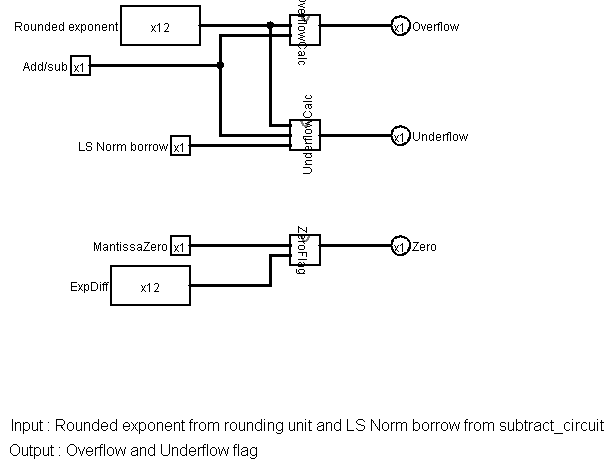
\includegraphics[scale=0.5]{Util/FlagUnit.png}
    \caption{Flag Unit.circ}
\end{figure}
\begin{figure}[!h]
    \centering
    \captionsetup{font=Large}
    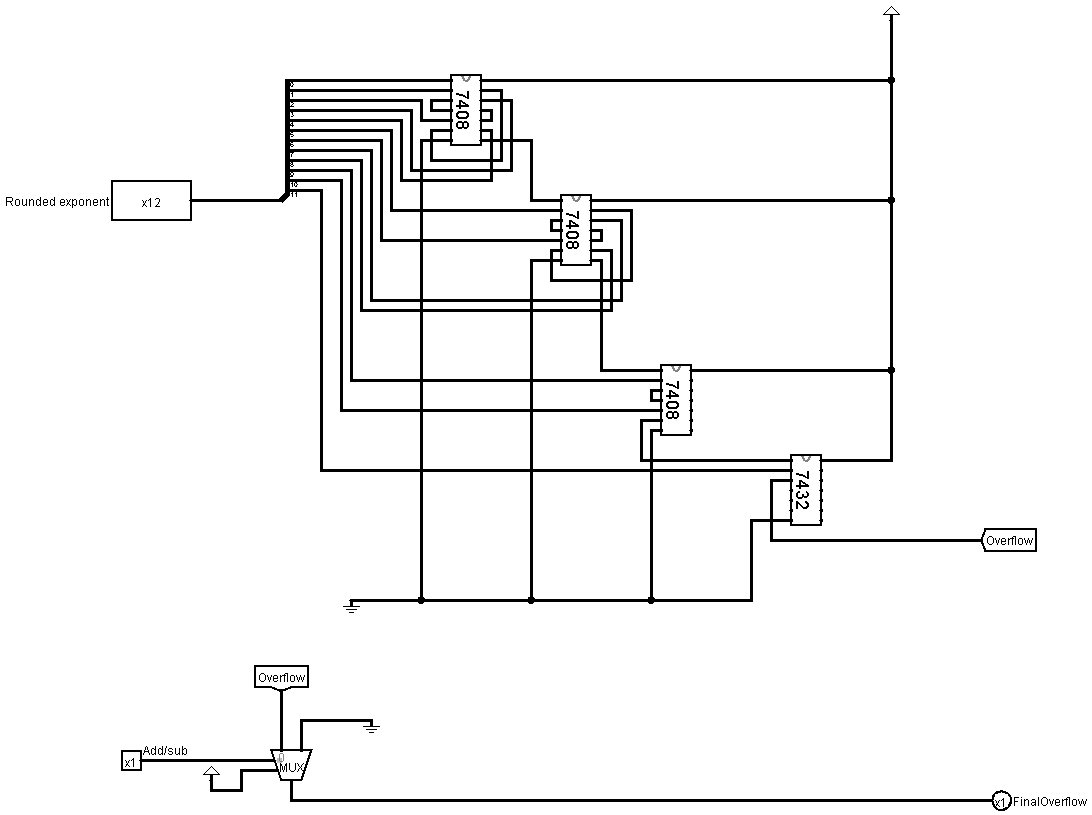
\includegraphics[scale=0.3]{Util/Overflow.png}
    \caption{Overflow.circ}
\end{figure}
\begin{figure}[t]
    \centering
    \captionsetup{font=Large}
    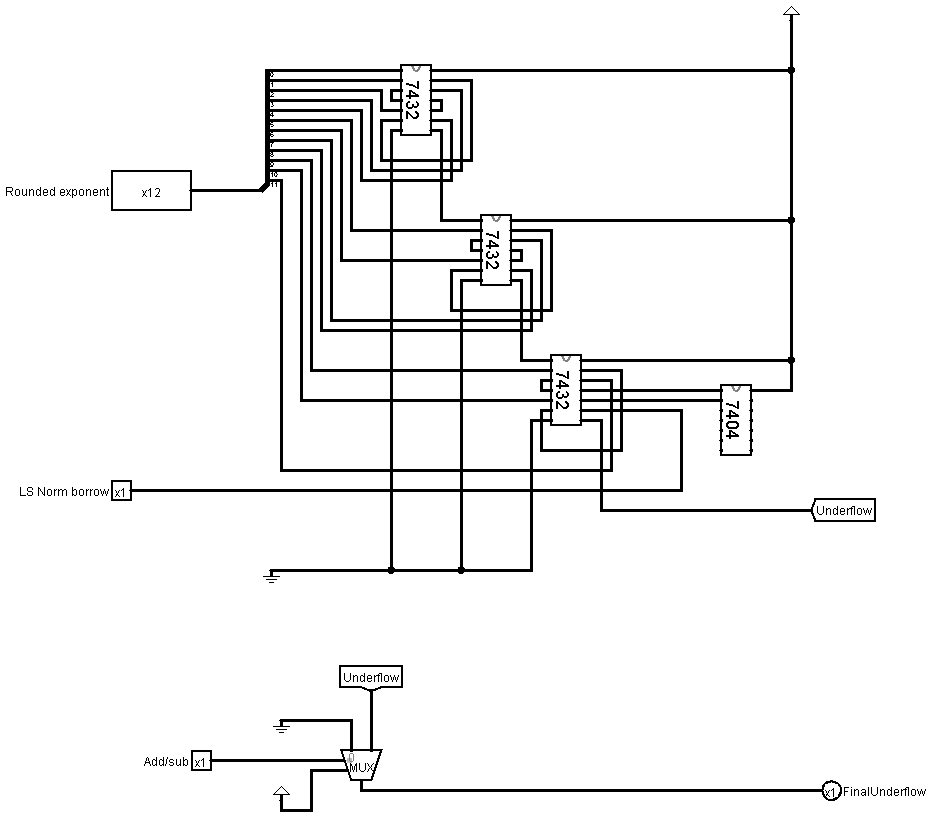
\includegraphics[scale=0.5]{Util/Underflow.png}
    \caption{Underflow.circ}
\end{figure}
\begin{figure}[!h]
    \centering
    \captionsetup{font=Large}
    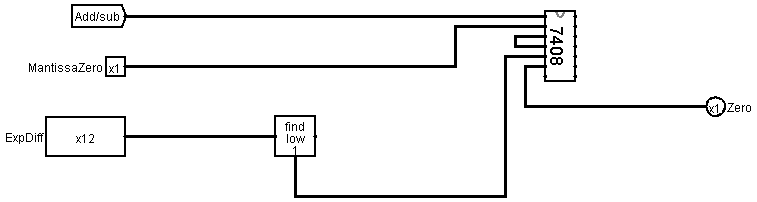
\includegraphics[scale=0.5]{Util/Zero.png}
    \caption{Zero.circ}
\end{figure}

\clearpage

\section{High-level Block Diagram of the Architecture}
\begin{figure}[!h]
    \centering
    \captionsetup{font=Large}
    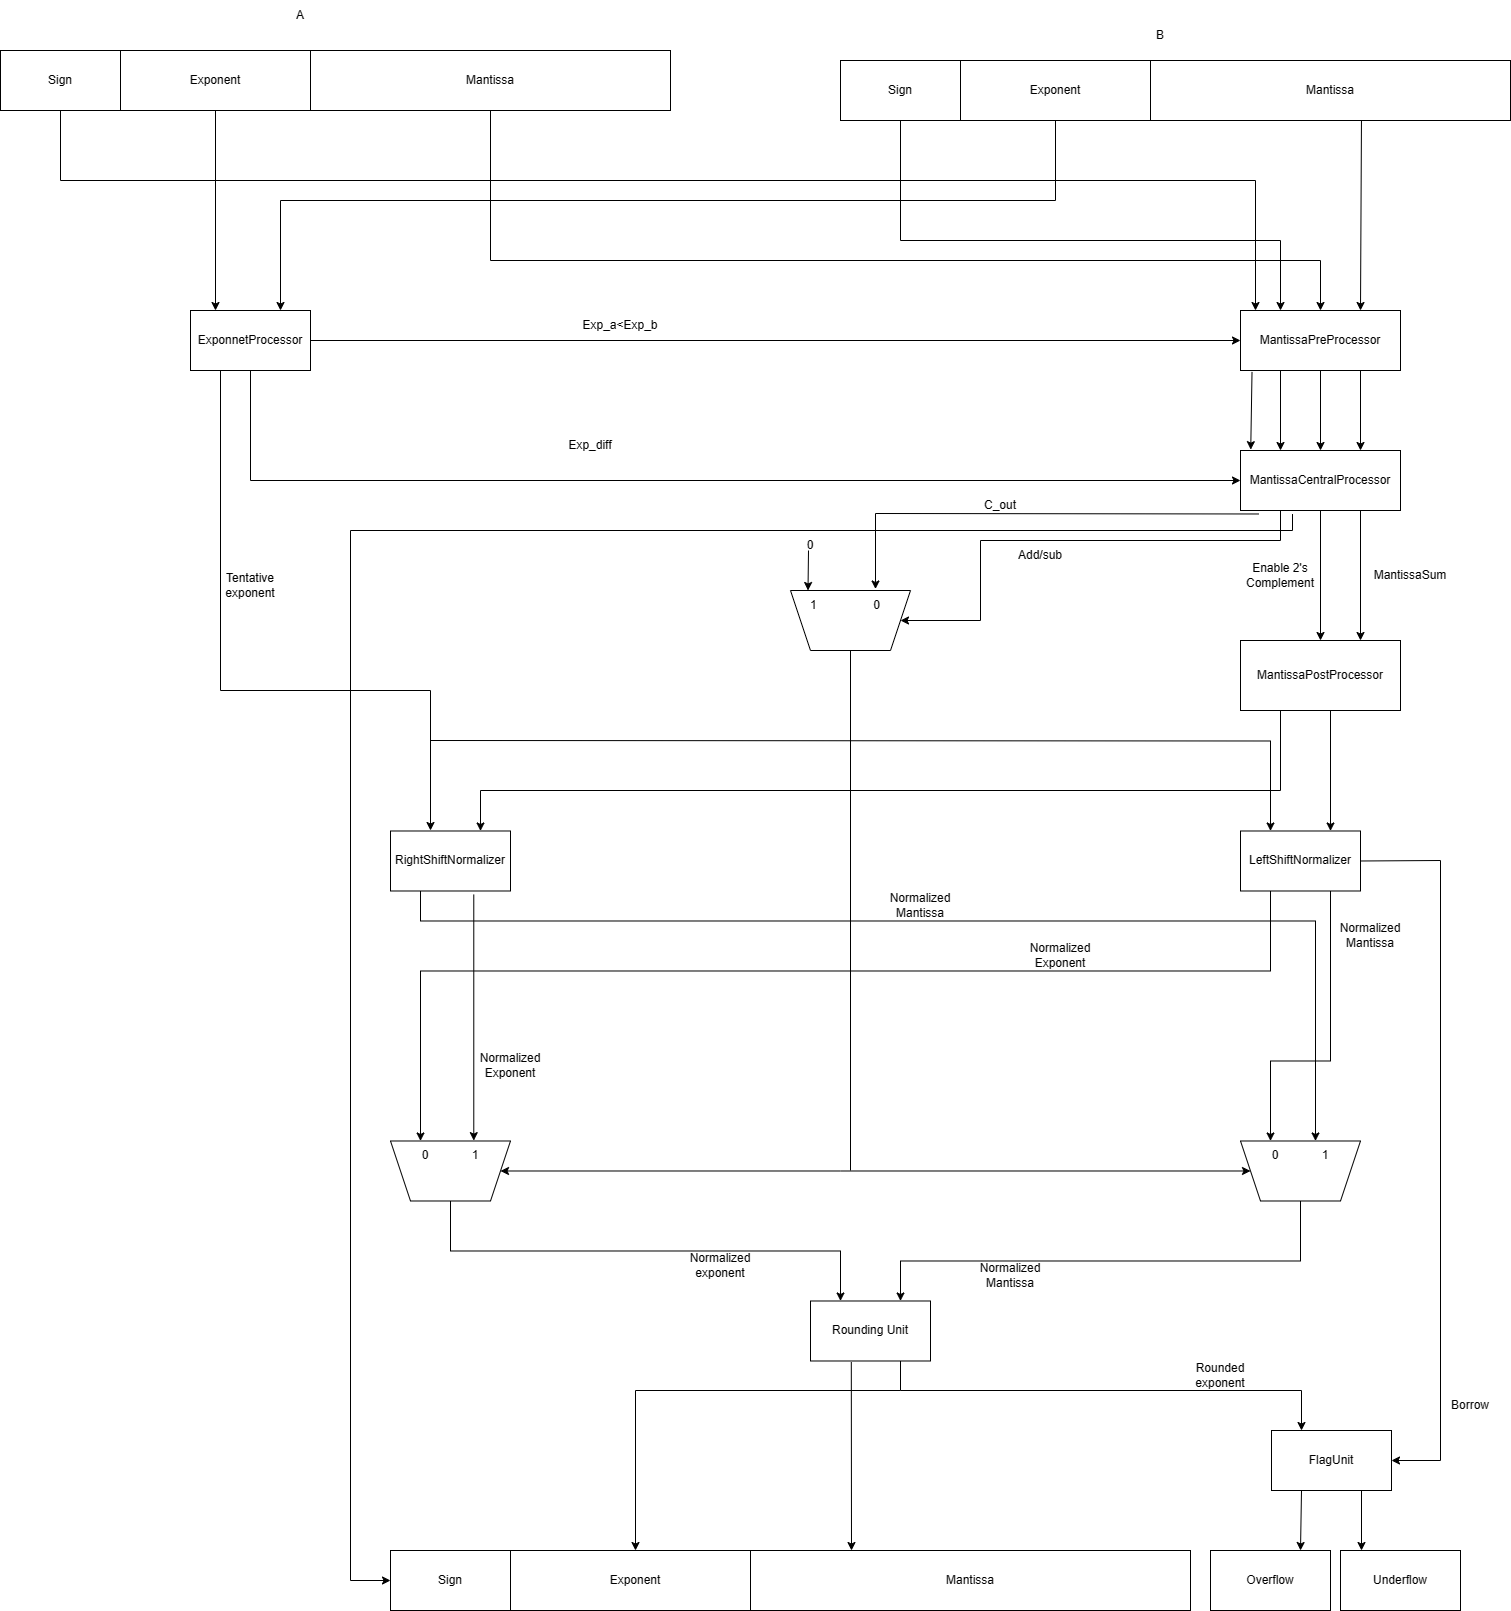
\includegraphics[width=\textwidth]{Util/block.png}
    \caption{High-level Block Diagram of the Architecture}
\end{figure}

\clearpage

\section{Design Description}
\subsection{Exponent Processing}
\Large
To add two floating-point numbers, the radix points must be aligned. This is typically done by shifting the input with the smaller exponent to the right to align it with the larger input. The exponent comparator circuit takes two exponents (12 bits) and give us which one is larger and which one is smaller.
 The exponent processor takes two exponents (12 bit) as input and calculates the difference of the exponents(12 bits). It also compares the two outputs and gives Ea<Eb(1 bit) as a flag. It also presents the larger exponent as the tentative exponent(12 bits).


\subsection{Rounding}
\Large
Our output floating point representation had 20 bits for mantissa. However, during our calculations, we extended the mantissa to 32 bits. Hence we rounded the final result to 20 bits. For rounding, we evaluated the 20th bit as Guard bit, 21th as Round bit. If any of the bits on the right of Round bit is set, the sticky bit would be set. Else, it is reset. So it it the logical \textbf{OR} operation of those bits. Based on the these bits as well as the 20th bit of the 32 bit mantissa from the normalizer module, we decide whether to round up or truncate based on the following truth table. 
\begin{table}[!h]
    \captionsetup{font=large}
    \centering
    \begin{tabular}{||c|c|c|c|c|c||}
    \hline
     $20th bit(P)$ & $G$ & $R$ & $S$ & $Decision$ & $RoundUp Flag(F)$ \\
     \hline
        X & 0 & X & X & Truncate & 0 \\
         \hline
        0 & 1 & 0 & 0 & Truncate & 0\\
        \hline
        1 & 1 & X & X & Round up & 1\\
        \hline 
        X & 1 & 1 & X & Round up & 1\\
        \hline 
        X & 1 & X & 1 & Round up & 1\\
        \hline
     
    \hline
    \end{tabular}
    \caption{Truth Table for rounding}
\end{table}
The round Up flag implies that we add 1 at the 20th bit when its set, else we truncate it. Moreover, when GRS = 100, we round to even, which implies that we add 1 if the 20th bit is set, rounding up to even. Else, we truncate it. 
\begin{figure}[!h]
    \captionsetup{font=large}
    \center{
    \begin{Karnaugh}
        \minterms{5,6,7,12,13,14,15}
        \maxterms{0,1,3,2,4,8,9,10,11}
        \implicant{5}{15}{orange}
        \implicant{7}{14}{yellow}
        \implicant{12}{14}{red}
    \end{Karnaugh}
    }
    \caption{K-Map for Round Up Flag(F)}
\end{figure}\\
From the K-map we get, $$F = G \land (P \lor R \lor S)$$
Also, we have to keep the mantissa normalized after rounding. If all of the 20 bits of the mantissa were to be 1, then on rounding up the floating point will be denormalized. To normalize it, we simply add one to the exponent and adjust it. Since all the bits would be reset in this case already, there is no need for right shift.
\subsection{Flag unit implementation}
In IEEE 754 format, range of exponent is -1022 to +1023. So, if the resultant exponent becomes less than -1022 (i.e. (exponent + bias) < 1), then it is underflow condition. Such condition can arise when (i) (exponent + bias) is 00000000000 or, (ii) less than 000000000. The (i) is detected by OR-ing all the bits of exponent and (ii) is deletected by checking the borrow from the subtractor used in left shifting normalization. The underflow flag is 1 when either of these conditions are met. And for overflow, the resultant exponent needs to be greater than 1023 (i.e. (exponent + bias) > 2046). Such condition can arise when (i) (exponent + bias) is 11111111111 or, (ii) greater than 11111111111. The (i) is detected by AND-ing all the bits of exponent and (ii) is deletected by checking the carry from the adder used in right shifting normalization. The overflow flag is 1 when either of these conditions is true. Also, when exponent becomes -1 (1111111111) in underflow condition, it fullfills the condition (i), even though it is not overflow. To handle this case, overflow flag is made 0 when two numbers with opposite signs are added.

\section{The Simulator Used along with the Version Number}

\Large

Logisim - 2.7.1

\newpage

\section{ICs used with count as a chart}

\begin{table}[!h]
    \captionsetup{font=Large}
    \centering
    \begin{tabular}{||c|c||}
    \hline
        \textbf{IC} & \textbf{Number of ICs} \\
        \hline
        7404 & 1 \\
        744075 & 2 \\
        7408 & 4 \\
        7432 & 4 \\
        7486 & 9 \\
    \hline
    \hline
        Total & 20 \\
    \hline
    \end{tabular}
    \caption{ICs and their number}
    \label{tab:ic-number}
\end{table}


\normalsize

\section{Discussion}
\Large
\justifying
The entire project was a pedagogic experience. Several difficulties had to be faced throughout the process.\par 
\vspace{5mm}
The circuit was significantly large. So, we implemented the fundamental units 
of the circuit as modules. Later, we assembled the entire circuit using these modules. This not only helped in the organization of the entire project but also facilitated the debugging process.
\par
\vspace{5mm}
In case of debugging, we extensively used the \textbf{probe} feature of \textbf{Logisim}. Also the circuit required an enormous amount of wire connections. This meant more chances of errors in the circuit. In addition, the debugging process would be tedious. To overcome these issues, we made ingenious use of the \textbf{tunnel} feature. Tunnel connects any two points with the same name. Firstly, this made our circuit organized and well-structured. Secondly, this eased the debugging process. Lastly, all the modules became easily interpretable.\par
\vspace{5mm}
We used the default adders, subtractors, multiplexers, and shifters provided with logisim as well as ICs from \textbf{7400-lib.circ}. The modules made optimum usage of both kinds of ICs.The default circuits aided in our design so that we could focus more on the main circuit. Even so, we implemented the smaller modules at IC level using the 7400 series ICs. Hence, we were able to learn and make the best usage of the tools available.In the end, we implemented the circuit judiciously.

\section{Contribution of Each Member}
\begin{itemize}
    \item 2005020 : Mostafa Rifat Tazwar 
    \begin{itemize}
        \item Circuit Design
        \begin{itemize}
            \item Arbitrary Right shifter
            \item Mantissa Pre and Post processor and debugging
            \item Rounding Unit
        \end{itemize}
        \item Report Writting
        \begin{itemize}
        \item Rounding
            \item Discussion
            \item Problem Specification
            \item Complete Report Organization
        \end{itemize}
    \end{itemize}
    \item 2005025 - Most. Sonia Khatun
    \begin{itemize}
        \item Circuit Design
        \begin{itemize}
        \item Left Shift normalization for subtraction  \item Right Shift normalization for addition
        \end{itemize}
    \end{itemize}
    \item 2005027 - Swastika Pandit
    \begin{itemize}
        \item Circuit Design
        \begin{itemize}
        \item Mantissa processing \item Flag unit \item Connecting the components to form complete circuit \item Circuit testing and debugging. 
        \end{itemize}
        \item Report Writing
        \begin{itemize}
            \item High level block diagram
			\item Circuit Diagram
            \item Flag Unit
        \end{itemize}
    \end{itemize}
    \item 2005029 - MD. Minhajul Islam Fuad
    \begin{itemize}
        \item Circuit Design
        \begin{itemize}
            \item Subtractor
        \end{itemize}
    \end{itemize}
    \item 2005030 - Fairuz Mubashwera
    \begin{itemize}
        \item Circuit Design
        \begin{itemize}
        \item Selecting the optimized choice for comparing/subtracting exponents
\item Building Exponent Processor and exponent comparator
\item Debugging and testing the circuit
        \end{itemize}
    \item Report Writting
        \begin{itemize}
        \item Introduction
        \item Flow Diagram
        \end{itemize}
    \end{itemize}
\end{itemize}

\end{document}